%% chapter02a_binary_strings_slides.tex
%% Beamer slides for Chapter 2 (Background), Section 2.1: Binary Strings
%% "An Introduction to Universal Artificial Intelligence"
%% by Marcus Hutter, Elliot Catt, and Jordi Grau-Moya (CRC Press / Chapman & Hall, 2024)
%% Reader-friendly style: complete sentences, symbol explanations, worked examples.
%% Compiled with: pdflatex -interaction=nonstopmode chapter02a_binary_strings_slides.tex  (twice)
\documentclass[aspectratio=169,10pt]{beamer}

\usetheme{Madrid}
\usecolortheme{seahorse}
\usefonttheme{professionalfonts}

%% ── Packages ──────────────────────────────────────────────────────────────
\usepackage{amsmath,amssymb,amsfonts}
\usepackage{mathtools}
\usepackage{graphicx}
\usepackage{booktabs}
\usepackage{array}
\usepackage{xcolor}
\usepackage{listings}

\graphicspath{{figures/}}

%% ── Python listing style ─────────────────────────────────────────────────
\lstdefinestyle{pycode}{
  language=Python,
  basicstyle=\ttfamily\scriptsize,
  numbers=left,
  numberstyle=\tiny\color{gray},
  frame=single,
  backgroundcolor=\color{gray!7},
  keywordstyle=\color{blue!70!black}\bfseries,
  commentstyle=\color{green!50!black}\itshape,
  stringstyle=\color{orange!80!black},
  showstringspaces=false,
  breaklines=true,
  tabsize=2,
  xleftmargin=1.0em,
  framexleftmargin=1.0em,
  aboveskip=4pt,
  belowskip=4pt,
}
\lstset{style=pycode}

%% ── Convenience macros ───────────────────────────────────────────────────
\newcommand{\Bs}{\mathbb{B}^{*}}
\newcommand{\Binf}{\mathbb{B}^{\infty}}
\newcommand{\Bb}{\mathbb{B}}
\newcommand{\len}{\ell}
\newcommand{\bij}[1]{\langle #1\rangle}

%% ── Metadata ─────────────────────────────────────────────────────────────
\title[UAI -- Ch.2.1]{An Introduction to Universal Artificial Intelligence}
\subtitle{Chapter 2: Background --- Section 2.1: Binary Strings}
\author{Based on Hutter, Catt \& Grau-Moya}
\institute{CRC Press / Chapman \& Hall, 2024}
\date{}

\setbeamertemplate{footline}[frame number]
\setbeamertemplate{navigation symbols}{}

%% ══════════════════════════════════════════════════════════════════════════
\begin{document}

\begin{frame}
  \titlepage
\end{frame}

\begin{frame}{Outline}
  \tableofcontents
\end{frame}

%% ══════════════════════════════════════════════════════════════════════════
\section{Chapter 2 Roadmap}
%% ══════════════════════════════════════════════════════════════════════════

\begin{frame}[allowframebreaks]{Chapter 2: Background --- What's in this Chapter?}

Chapter 2 is an \emph{optional} chapter that collects all the prerequisite
mathematics used by the rest of the book. If you already know a topic, skip
its section; if you find a gap, come back here. Below is a plain-English
tour of every section, quoting the epigraph the authors chose:

\begin{quote}
\itshape ``Give me six hours to chop down a tree and I will spend the first
four sharpening the axe.'' \hfill --- Abraham Lincoln
\end{quote}

\textbf{2.1 Binary Strings} (this deck). Defines strings and the operations
on them, self-delimiting prefix codes, and the cylinder sets used later to
put probability measures on infinite sequences.

\framebreak

\textbf{2.2 Measure Theory and Probability Theory.} States the axioms of
probability, defines (semi)measures on infinite sequences, conditional
probability, random variables, expectation and variance, key probability
inequalities, and convergence of random variables.

\textbf{2.3 Statistical Inference and Estimation.} Introduces the
``sunrise problem,'' maximum likelihood estimation, and the notion of a
consistent estimator --- one that learns the truth given enough data.

\textbf{2.4 Bayesian Probability Theory.} Derives Bayes' theorem, Bayesian
estimation and prediction, and the classical Laplace rule for predicting
binary sequences.

\framebreak

\textbf{2.5 Information Theory and Coding.} Covers Shannon entropy, the
Shannon--Fano and arithmetic codes, the Kullback--Leibler divergence, the
Kraft inequality, and Shannon's coding theorem --- the mathematics of how
few bits a message truly needs.

\textbf{2.6 Computability Theory.} Formal models of computation, the
Halting Problem, semi-computable functions, and the arithmetic hierarchy
--- the mathematics of what can and cannot be computed at all.

\framebreak

\textbf{2.7 Kolmogorov Complexity.} Measures the intrinsic complexity of a
string (rather than the randomness of the process that produced it),
giving a rigorous formalization of ``simplicity'' and hence of Occam's
razor. Connects to the Minimum Description Length principle and to
Shannon entropy.

\textbf{2.8 Miscellaneous.} Distances between probability distributions
(total variation, squared, Kullback--Leibler, Hellinger), how to handle
semimeasures (probability that can ``leak away''), and how to condition on
probability-zero events.

\textbf{2.9 History and References.} Pointers to the literature.

\framebreak

\textbf{Why start with binary strings?} Section 2.1 introduces the
fundamental concept of strings and their binary encoding through prefix
codes, which allows unique recovery of concatenated and transmitted
strings. Every later formal object in the book --- programs, data,
observations, hypotheses --- is ultimately represented as a binary string,
so we need to fix this notation precisely before anything else.

\end{frame}

%% ══════════════════════════════════════════════════════════════════════════
\section{2.1 Binary Strings: Motivation}
%% ══════════════════════════════════════════════════════════════════════════

\begin{frame}{2.1 Binary Strings}
We assume a brief familiarity with set theory, real analysis, metric
spaces, norms, and topological spaces. Often we take these mathematical
structures for granted, but to \emph{prove} properties about them later in
the book we need a formal definition of every object we use --- mathematics
provides the tools of rigor that let us do this without endless
philosophical discussion.

\vspace{0.4cm}
\textbf{In this section we define:}
\begin{itemize}
  \item strings and the operations defined on them (2.1.1),
  \item self-delimiting \emph{prefix codes} (2.1.2),
  \item and \emph{cylinder sets}, used later to put probability measures on
    infinite binary sequences (2.1.3).
\end{itemize}
\end{frame}

%% ══════════════════════════════════════════════════════════════════════════
\subsection{2.1.1 Finite Binary Strings and Natural Numbers}
%% ══════════════════════════════════════════════════════════════════════════

\begin{frame}{2.1.1 Finite Binary Strings $\Bs$ and Natural Numbers $\mathbb{N}_0$}

We define $\Bb^n$ as the set of all binary strings of length $n$ (all
sequences of $n$ zeros and ones). The set of all finite strings over
$\Bb=\{0,1\}$ is defined as
\[
  \Bs \;:=\; \bigcup_{n=0}^{\infty}\Bb^{n} \;=\;
  \{\epsilon,\, 0,\, 1,\, 00,\, 01,\, 10,\, 11,\, 000,\, \dots\}.
\]
\textbf{Plain English.} $\Bb^n$ is ``all bit patterns of exactly $n$ bits''
(e.g.\ $\Bb^2=\{00,01,10,11\}$). Taking the union over every length $n\geq0$
gives $\Bs$, the set of \emph{all} finite bit strings, including the
\emph{empty string} $\epsilon$ (length $0$, no bits at all).

\medskip
We typeset bits in \texttt{monospace} to distinguish them from numbers:
\texttt{101} is the binary string one-zero-one, while $101$ is the number
``one-hundred-and-one.''

\medskip
For two strings $x=x_1x_2x_3\dots x_n$ and $y=y_1y_2y_3\dots y_m$, the
\textbf{concatenation} is
\[
  xy \;:=\; x_1x_2x_3\dots x_n\, y_1y_2y_3\dots y_m ,
\]
i.e.\ writing $y$ right after $x$. Clearly $\Bs$ is closed under
concatenation (gluing two finite strings gives another finite string). The
set of \emph{infinite} binary sequences is denoted $\Binf$ (studied in
2.1.3).
\end{frame}

\begin{frame}{Notation for Bits, Substrings, and Length}

By convention we use \emph{string} or \emph{word} for an element of $\Bs$.
For example, $x=x_1x_2x_3\dots x_n$ is a finite binary string of length $n$.

\begin{itemize}
  \item The \textbf{$i$th bit} of $x$ is denoted $x_i$, for $1\leq i\leq
    \len(x)$, where $\len:\Bs\to\mathbb{N}_0$ maps a string to its length
    (number of bits it contains), e.g.\ $\len(x_{1:n})=n$.
  \item Given $i,j$ with $1\leq i\leq j\leq n$, the \textbf{substring}
    $x_{i:j}$ (pronounced ``$x$ from $i$ to $j$'') is the length-$(j-i+1)$
    segment $x_ix_{i+1}\dots x_j$. For $j<i$ we define $x_{i:j}=\epsilon$
    (an empty segment).
  \item Shorthand: $x_{1:n}$ and $x_{\leq n}$ both mean $x_1x_2x_3\dots
    x_n$; $x_{<n}$ means $x_1x_2x_3\dots x_{n-1}$ (everything strictly
    before position $n$).
  \item Each binary digit is called a \textbf{bit}. The empty string
    $\epsilon$ has length $\len(\epsilon)=0$.
\end{itemize}

\medskip
We also use the standard sets: $\mathbb{R}$ (real numbers), $\mathbb{Q}$
(rationals), and $\mathbb{N}_0=\{0,1,2,\dots\}$ (natural numbers
\emph{including} zero).
\end{frame}

\begin{frame}{Interpreting a String as a Number}

The standard way to read a binary string as a number in base 2 is
\[
  b(x) \;:=\; \sum_{i=1}^{\len(x)} 2^{\len(x)-i}\,[\![x_i=1]\!]
\]
\textbf{Plain English.} $b(x)$ ``reads off'' $x$ as an ordinary binary
number: the bracket $[\![x_i=1]\!]$ equals $1$ if bit $x_i$ is a \texttt{1}
and $0$ otherwise, and $2^{\len(x)-i}$ is the place-value (like the
``tens,'' ``hundreds,'' etc.\ columns, but in base 2) of the $i$th bit. For
example, $b(\texttt{00101})=5$ (interpreting \texttt{00101} in binary), and
$b(\epsilon)=0$ (empty sum).

\medskip
\textbf{The catch: $b$ is not a bijection.} Leading zeros are invisible to
$b$ --- e.g.\ $b(\texttt{101})=b(\texttt{0101})=5$ --- so different strings
map to the same number, and $b$ cannot be inverted.

\medskip
\textbf{The fix.} We build a genuine one-to-one correspondence
$\bij{\cdot}:\Bs\to\mathbb{N}_0$ between strings and natural numbers by
mapping $x$ to the number whose binary representation is $\texttt{1}x$
(prefix a leading \texttt{1} to kill the ambiguity), then subtracting $1$
so that the empty string maps to $0$:
\[
  \bij{x} \;=\; b(1x) - 1 .
\]
\end{frame}

\begin{frame}{The Bijection $\bij{\cdot}$: Examples}

For example, the string \texttt{01} maps to $b(101)-1 = 5-1 = 4$ under this
bijection. Some more examples of the bijective mapping $\bij{\cdot}$ for
strings in $\Bs$:

\begin{center}
\begin{tabular}{c|c|c|c|c|c|c|c|c|c|c}
$\Bs$ & $\epsilon$ & \texttt{0} & \texttt{1} & \texttt{00} & \texttt{01} &
  \texttt{10} & \texttt{11} & \texttt{000} & \texttt{001} & $\dots$ \\
\hline
$\mathbb{N}_0$ & 0 & 1 & 2 & 3 & 4 & 5 & 6 & 7 & 8 & $\dots$
\end{tabular}
\end{center}

\textbf{Plain English.} Reading down the table: the strings are enumerated
first by increasing length, then lexicographically ($0$ before $1$) within
each length --- exactly the order you'd count in binary if you started at
$0$ and never worried about leading zeros.
\end{frame}

\begin{frame}{Proposition 2.1.1: Canonical Bijection from $\Bs$ to $\mathbb{N}_0$}

\begin{block}{Proposition 2.1.1 (Canonical bijection from $\Bs$ to $\mathbb{N}_0$)}
Let $x$ be a binary string. Define
\[
  \bij{x} \;:=\; 2^{\len(x)} + b(x) - 1 \qquad\text{with}\qquad
  b(x) \;:=\; \sum_{i=1}^{\len(x)} 2^{\len(x)-i}\,[\![x_i=1]\!].
\]
Then $\bij{\cdot}$ is a bijective map, and it enumerates $\Bs$, sorted
first by length, then lexicographically.
\end{block}

\textbf{Plain English.} This is the same formula as before, just expanded:
since prefixing a \texttt{1} to $x$ multiplies every place value by $2$ and
adds one more $2^{\len(x)}$ term, $b(1x)=2^{\len(x)}+b(x)$, matching
$\bij{x}=b(1x)-1$ from the previous slide. \emph{Bijective} means every
natural number corresponds to exactly one string, and vice versa --- no
number is missed, and none is hit twice.

\medskip
\textbf{Proof.} Left as an exercise to the reader (in the book).
\end{frame}

\begin{frame}{The Inverse Bijection, and Dropping the Notation}

The inverse of this bijection can be written as
\[
  \bij{n}^{-1} \;=\; b^{-1}_{\lfloor\log_2(n+1)\rfloor}\bigl(n+1-2^{\lfloor\log_2(n+1)\rfloor}\bigr)
  \tag{2.1.2}
\]
\textbf{Plain English.} $b_k^{-1}(n)$ takes a natural number $n$ and
returns a string of $k$ bits representing $n$ in binary with no leading
zeros for positive numbers, padded with leading zeros to reach length $k$
(e.g.\ $b_5^{-1}(7)=\texttt{00111}$); $b_k^{-1}(n)$ is left undefined if $k$
is too small to fit $n$'s binary encoding. This ensures the encoded string
satisfies $\len(\bij{n}^{-1})=\lfloor\log_2(n+1)\rfloor$. One can verify
this is the valid inverse of $\bij{\cdot}$ by rearranging the formula for
$\bij{x}$ and substituting $\len(x)=\lfloor\log_2(n+1)\rfloor$.

\medskip
\textbf{A notational convenience used throughout the book:} once the
bijection is fixed, we often \emph{drop} it and let context decide whether
a symbol is a string or a number. For instance, we may write $x+1$ instead
of $\bij{x}+1$ when $x$ is a string, or $\len(n)$ instead of
$\len(\bij{n}^{-1})$ for a natural number $n$.
\end{frame}

\begin{frame}{Proposition 2.1.3: How Big is $\bij{x}$?}

\begin{block}{Proposition 2.1.3 (Bijection length bound)}
Let $x$ be a binary string. Then
\[
  2^{\len(x)} - 1 \;\leq\; \bij{x} \;\leq\; 2^{\len(x)+1} - 2 .
\]
\end{block}

\textbf{Plain English.} The number $\bij{x}$ that a length-$\len(x)$ string
maps to is always roughly $2^{\len(x)}$ --- squeezed between
$2^{\len(x)}-1$ (when $x$ is all zeros) and $2^{\len(x)+1}-2$ (when $x$ is
all ones). In other words, a string's numeric ``address'' grows
\emph{exponentially} with its length.

\medskip
\textbf{Proof.} Note that $0\leq b(x)\leq 2^{\len(x)}-1$ (the smallest
value of $b(x)$ is $0$, all-zero string; the largest is $2^{\len(x)}-1$,
all-one string), from which the result follows by substituting into
$\bij{x}=2^{\len(x)}+b(x)-1$. $\blacksquare$

\medskip
This exponential growth is exactly what makes the ``zeroth-order'' prefix
code inefficient, as we will see in Section 2.1.2.
\end{frame}

%% ══════════════════════════════════════════════════════════════════════════
\begin{frame}[fragile]{Python: The Bijection $\bij{\cdot}$ Between Strings and Numbers}

We implement $b(x)$, the bijection $\bij{\cdot}$, and its inverse, and
check them against the table of examples above.

\begin{lstlisting}
def b(x):
    """Interpret binary string x as a base-2 number (leading zeros lost)."""
    return int(x, 2) if x != "" else 0

def bij(x):
    """Canonical bijection <.>: B* -> N0.  <x> = b(1x) - 1."""
    return b("1" + x) - 1

def bij_inv(n):
    """Inverse of bij: N0 -> B*."""
    k = (n + 1).bit_length() - 1        # k = floor(log2(n+1))
    rest = n + 1 - 2 ** k                # the part after the leading 1
    return format(rest, "0{}b".format(k))  # k bits, zero-padded

for s in ["", "0", "1", "00", "01", "10", "11", "000", "001"]:
    print(f"<{s!r:>6}> = {bij(s)}   inverse: {bij_inv(bij(s))!r}")
\end{lstlisting}

\textbf{Output (first few rows):}
\texttt{<''> = 0, <'0'> = 1, <'1'> = 2, <'00'> = 3, <'01'> = 4, <'10'> = 5,
<'11'> = 6, <'000'> = 7, <'001'> = 8} --- exactly matching the table.
\end{frame}

%% ══════════════════════════════════════════════════════════════════════════
\subsection{2.1.2 Prefix Codes}
%% ══════════════════════════════════════════════════════════════════════════

\begin{frame}{Why We Need Prefix-Free Codes}

Often, when transmitting a message across a medium, the message is
converted into a sequence of symbols called a \textbf{code}, which is then
transmitted and decoded to recover the original message. A binary code is
ideal since it needs only two distinct symbols --- but this is problematic
if we want to send \emph{multiple} messages.

\medskip
\textbf{The ambiguity problem.} Suppose we want to transmit the sequence of
numbers $(1,3)$. We encode each number using the bijection, $\bij{1}=0$ and
$\bij{3}=00$, and transmit the concatenation $\bij{1}\bij{3}=\texttt{000}$.
The receiver knows the code, but this is ambiguous: \texttt{000} could be
decoded as $(3,1)$, $(1,1,1)$, or $(1,3)$.

\medskip
\textbf{A bad fix.} We could add a delimiter symbol \texttt{\#} and
transmit \texttt{0\#00} --- but now we have wasted an extra symbol, which
itself needs encoding if we want to transmit \emph{only} binary strings.

\medskip
\textbf{The real solution.} Restrict the allowed encodings to a
\textbf{prefix-free} set of binary strings: a set in which no member is a
prefix of another. This makes every encoded message \emph{uniquely
decodable}, with no delimiter needed.
\end{frame}

\begin{frame}{Definitions: Prefix, Prefix-Free, Prefix Code}

Let $x,y\in\Bs$ be strings.

\begin{itemize}
  \item We say $x$ is a \textbf{prefix} of $y$ (denoted $x\sqsubseteq y$)
    if $\exists z\in\Bs$ such that $xz=y$ (i.e.\ $y$ starts with $x$, and
    the rest is $z$).
  \item If additionally $z\neq\epsilon$, we call $x$ a \textbf{proper
    prefix} of $y$ (denoted $x\sqsubset y$) --- $x$ is a strictly shorter
    initial segment of $y$.
  \item A set $\mathcal{P}\subseteq\Bs$ is \textbf{prefix-free} if no
    element of the set is a proper prefix of another.
  \item Given an injection $c:\Bs\to\Bs$ (a function that never maps two
    different inputs to the same output), if $\{c(x):x\in\Bs\}$ is
    prefix-free, we call $c$ a \textbf{prefix-code}. The elements of
    $\mathcal{P}$ are called \textbf{(prefix) codewords}.
\end{itemize}

\medskip
\textbf{Why this matters.} Using prefix codes, a message is always
\emph{uniquely decodable} --- there is no ambiguity in decoding, unlike the
$\bij{1}\bij{3}$ example above. The message can be transmitted as a
sequence of concatenated codewords with \emph{no} reserved delimiter symbol
needed to separate the words.

\medskip
\textbf{A real-world non-example: Morse code.} Morse code
$\{\texttt{-}\!\cdot\!\cdot,\ \texttt{-}\!-\}$ is \emph{not} a prefix code,
as \texttt{-.--} could be decoded as any of
$\{$Y, KT, NTT, NM, TAT, TW, TEM, TETT$\}$. (Morse code actually uses three
symbols --- a space, plus the absence versus presence of a pulse --- and
adds spaces between letters as a delimiter.)
\end{frame}

\begin{frame}{Prefix Codes as Binary Trees}

\begin{center}
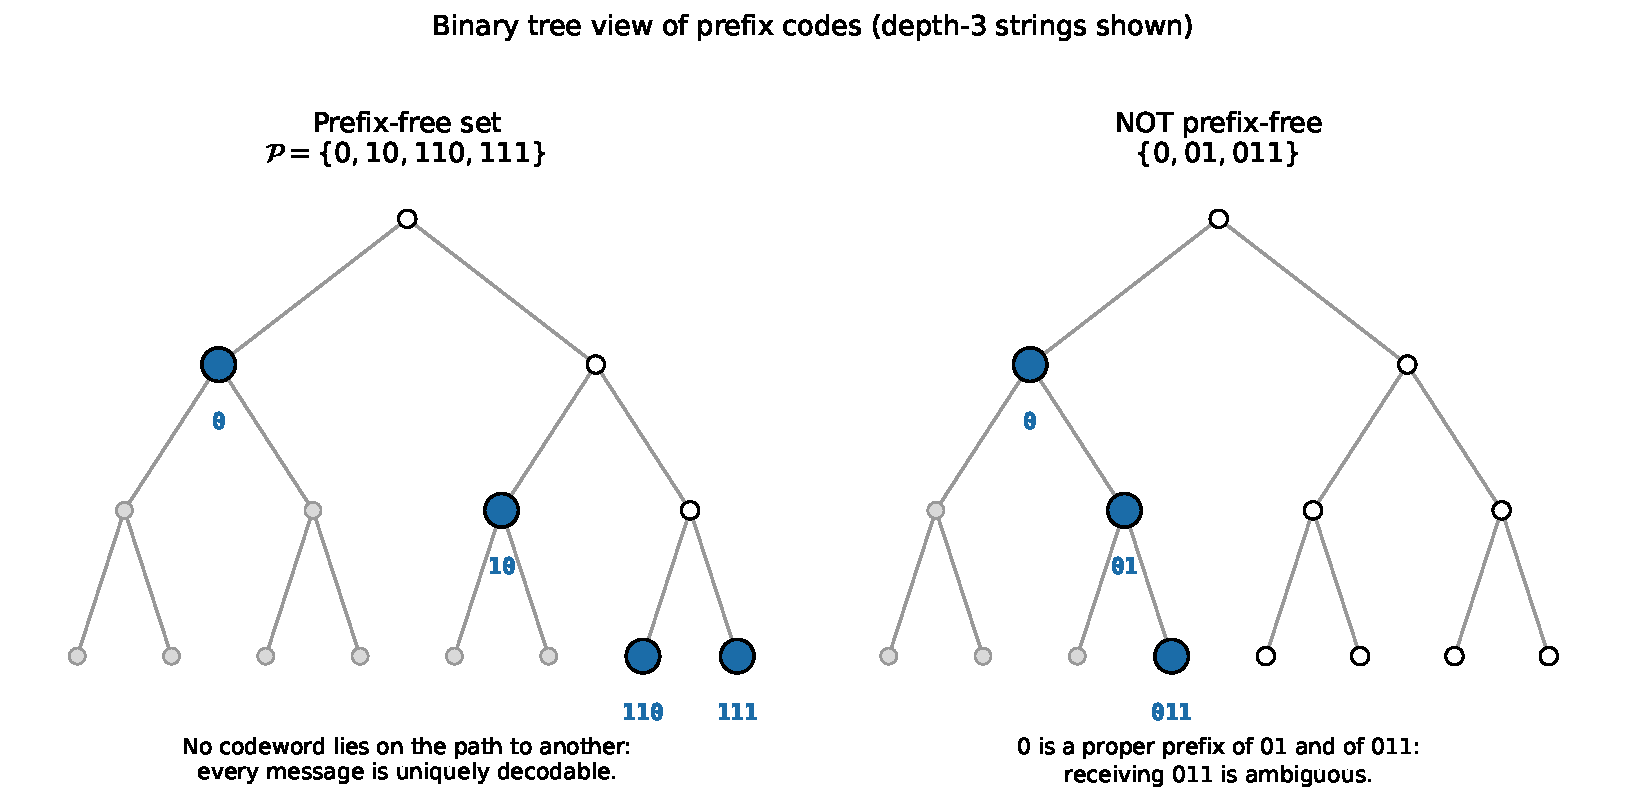
\includegraphics[width=0.78\textwidth]{fig_binary_tree}
\end{center}

\centering Choosing a codeword ``cuts'' its branch of the tree, blocking
every string below it from also being a codeword.
\end{frame}

\begin{frame}{Reading the Prefix-Code Tree}

\textbf{Plain English.} Think of $\Bs$ as a binary tree: the root is
$\epsilon$, and each node $x$ has two children, $x\texttt{0}$ and
$x\texttt{1}$. Choosing a codeword $x$ ``cuts'' that branch --- every
string below $x$ in the tree (every string that has $x$ as a proper
prefix) becomes unusable as a codeword, since it would collide with $x$.

\medskip
A set is prefix-free exactly when no codeword lies on the tree-path to
another, as in $\mathcal{P}=\{0,10,110,111\}$ on the left of the previous
figure. The set $\{0,01,011\}$ on the right fails: $0$ is a proper prefix
of both $01$ and $011$, so seeing \texttt{0} arrive does not tell the
receiver whether the message is finished or two more bits are coming.
\end{frame}

\begin{frame}{Building an Infinite Family of Prefix Codes}

There are (uncountably) many ways to construct prefix codes in $\Bs$. One
can construct an infinite family of prefix codes $E_i$ for $\Bs$ by
defining, for a string $x\in\Bs$, its \textbf{$i$th-order prefix codeword}
recursively as
\[
  E_i(x) \;=\;
  \begin{cases}
    1^{x}0 & i=0 \\
    E_{i-1}(\len(x))\,x & \text{otherwise}
  \end{cases}
  \tag{2.1.4}
\]
where $1^n$ denotes the string $111\dots1$ of $n$ ones (not to be confused
with $1$ raised to the power of $n$). We call $E_i(x)$ a
\textbf{self-delimiting encoding} of $x$.

\medskip
\textbf{Plain English, base case ($i=0$).} $1^x0$ means: write the digit
\texttt{1}, repeated $\bij{x}$ many times (recall we drop $\bij{\cdot}$ in
the exponent, per the earlier convention), followed by a single
\texttt{0}. The ending \texttt{0} acts as a delimiter, so if many
zeroth-order codewords are concatenated, we can always tell where one ends
and the next begins.

\medskip
\textbf{Recursive case ($i\geq1$).} To encode $x$ at order $i$, first
self-delimit its \emph{length} $\len(x)$ at order $i-1$, then simply append
$x$ itself (no further delimiter is needed, because we now already know
how many bits of $x$ to read).
\end{frame}

\begin{frame}{Zeroth-Order Code: Simple but Wasteful}

Despite its simplicity, the zeroth-order prefix code $E_0$ is undesirable:
its codewords are much longer than the original message, making it
inefficient for practical data transmission. By Proposition 2.1.3,
\[
  \len(E_0(x)) \;=\; \bij{x}+1 \;=\; O\bigl(2^{\len(x)}\bigr),
\]
which grows \textbf{exponentially} with the length of $x$.

\textbf{Plain English.} Encoding a message of, say, $20$ bits this way
could require over a \emph{million} bits --- clearly undesirable. We would
prefer an encoding with length approximately equal to $\len(x)$, with
minimal overhead. (The code cannot map \emph{every} string $x$ to a
codeword shorter than $\len(x)$: that would give an injection from $\Bb^n$
to $\Bb^{<n}$, which is impossible by a simple counting argument, since
$\Bb^{<n}$ has fewer than $2^n$ elements.) Due to this, we often resort to
a \emph{higher-order} prefix code.
\end{frame}

\begin{frame}{First- and Second-Order Prefix Codes}

We often use the \textbf{first-order prefix code} $\overline{x}$ of $x$:
\[
  \overline{x} \;:=\; E_1(x) \;=\; E_0(\len(x))\,x \;=\; 1^{\len(x)}0\,x .
\]
\textbf{Plain English.} First self-delimit the \emph{length} of $x$ using
the (wasteful, but now applied to a much smaller number) zeroth-order
code, then append $x$ itself.

\medskip
And the \textbf{second-order prefix code} $x'$ of $x$:
\[
  x' \;:=\; E_2(x) \;=\; E_1(\len(x))\,x \;=\; \overline{\len(x)}\,x \;=\;
  1^{\len(\len(x))}0\,\len(x)\,x .
\]
\textbf{Plain English.} Self-delimit the length of $x$ using the
\emph{first}-order code instead --- cheaper still, because now even the
wasteful part ($1^{\len(\len(x))}0$) is applied to the tiny number
$\len(\len(x))$.

\medskip
\emph{Footnote (notation subtlety).} Strictly, $\len$ cannot be composed
with itself since $\len:\Bs\to\mathbb{N}_0$ takes a string and returns a
number, not a string; formally one should write
$x'=\overline{\bij{\len(x)}^{-1}}\,x$. We keep $\bij{\cdot}$ implicit
throughout, exactly as promised earlier.

\medskip
Higher-order prefix codes offer diminishing returns and are seldom used.
\end{frame}

\begin{frame}{How Much Overhead Do $\overline{x}$ and $x'$ Add?}

The lengths of $\overline{x}$ and $x'$ are bounded as follows:
\begin{align}
  \len(\overline{x}) &= 2\len(x)+1 \notag\\
  \len(x') &= \len(x) + 2\len(\len(x)) + 1 \notag\\
  &= \len(x) + 2\log_2(\len(x)) + O(1).
  \tag{2.1.5}
\end{align}

\textbf{Plain English.} $\overline{x}$ adds at most $2\log_2\len(x)$ bits
of overhead to the length of $x$ (since $\len(x)\leq2^{\len(\len(x))}$ by
Proposition 2.1.3, so $\len(\len(x))=O(\log_2\len(x))$); and $x'$ adds only
$\log_2\len(x) + 2\log_2\log_2\len(x)$ overhead. Both grow as
$O(\log_2\len(x))$ --- a modest penalty compared to the length of the
message itself, unlike the exponential blow-up of $E_0$.
\end{frame}

\begin{frame}{Overhead in Pictures: $E_0$ vs.\ $\overline{x}$ vs.\ $x'$}

\begin{center}
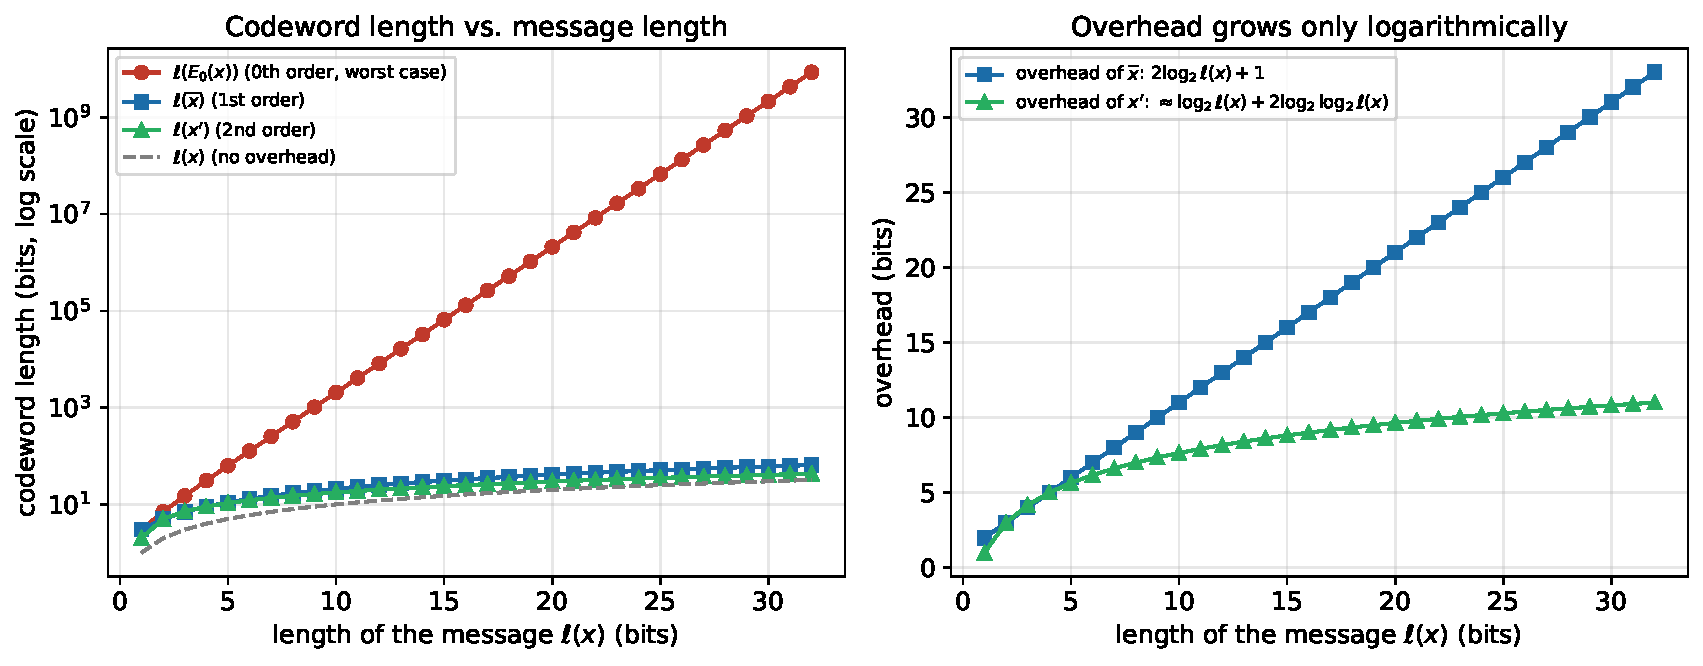
\includegraphics[width=0.85\textwidth]{fig_code_length_growth}
\end{center}

\centering \footnotesize
Left: $E_0$ grows exponentially in $\len(x)$ while $\overline{x}$ and $x'$
track $\len(x)$ closely. Right: the overhead of $\overline{x}$ and $x'$
alone, both $O(\log_2\len(x))$.
\end{frame}

\begin{frame}{Lemma 2.1.6 and Theorem 2.1.7}

\begin{block}{Lemma 2.1.6 ($i$th-order code is prefix)}
$E_i(\cdot)$ is a prefix code for all $i\in\mathbb{N}_0$.
\end{block}

\textbf{Proof idea.} The case $i=0$ was discussed above (the trailing
\texttt{0} delimits). For $i=1$: suppose $\overline{x}$ were a proper
prefix of $\overline{y}$ for $x\neq y$, i.e.\ $\overline{x}z=\overline{y}$
for some $z\neq\epsilon$. Then $1^{\len(x)}0xz=1^{\len(y)}0y$; the strings
must agree up to the first zero, forcing $\len(x)=\len(y)$; but then
$\len(x)+\len(z)=\len(\overline{x}z)=\len(\overline{y})=\len(x)$, forcing
$\len(z)=0$, i.e.\ $z=\epsilon$, a contradiction. The proof for $i>1$
follows by induction.

\begin{block}{Theorem 2.1.7 (Uniqueness of prepending prefix codes)}
For any two given strings $x,y\in\Bs$ and any prefix code $c$, $c(x)y$ is
uniquely decodable.
\end{block}

\textbf{Plain English \& proof idea.} Since $c$ is a prefix code, the
prefix of $c(x)y$ that lies in the range of $c$ must be \emph{unique}
(because $c(x)$ is in the range of $c$, we can separate $c(x)y$ into
$c(x)$ and $y$ unambiguously). We can then recover $x$ from $c(x)$, and
whatever remains is $y$. This motivates encoding a \emph{pair} of strings
$(x,y)$ as $\overline{x}y$ or $x'y$ --- leaving the \emph{last} string
unencoded saves bits versus encoding both, e.g.\ $\overline{x}\,\overline{y}$.
\end{frame}

%% ══════════════════════════════════════════════════════════════════════════
\begin{frame}[fragile]{Python: Building Self-Delimiting Codes}

We implement $E_0$ and the first-order code $\overline{x}$ directly from
definition (2.1.4).

\begin{lstlisting}
def E0(x):
    """Zeroth-order self-delimiting code: 1^<x> 0."""
    n = bij(x)                 # <x>, the bijection defined earlier
    return "1" * n + "0"

def xbar(x):
    """First-order code: E0(len(x)) x = 1^len(x) 0 x."""
    return "1" * len(x) + "0" + x

print("E0('01')   =", E0("01"))     # <01> = 4  ->  "11110"
print("xbar('101') =", xbar("101")) # len=3     ->  "1110101"
\end{lstlisting}

\textbf{Output:} \texttt{E0('01') = 11110}, \texttt{xbar('101') = 1110101}
--- matching $\len(\overline{x})=2\len(x)+1=7$ from (2.1.5).
\end{frame}

\begin{frame}[fragile]{Python: Verifying Unique Decodability (Theorem 2.1.7)}

We now check that concatenating a first-order codeword with an unencoded
string, $\overline{x}y$, is uniquely decodable with no delimiter needed.

\begin{lstlisting}
def decode_pair(code):
    """Decode xbar(x) y  ->  (x, y), Theorem 2.1.7 in action."""
    n = code.index("0")         # position of first 0 = len(x)
    x = code[n + 1 : n + 1 + n]  # len(x) was unary-coded before the 0
    y = code[n + 1 + n :]
    return x, y

x, y = "101", "0011"
transmitted = xbar(x) + y
print("transmitted =", transmitted)
print("decoded     =", decode_pair(transmitted), " expected =", (x, y))
\end{lstlisting}

\textbf{Output:} \texttt{transmitted = 11101010011},
\texttt{decoded = ('101', '0011') = expected} --- confirming that
$\overline{x}y$ is uniquely decodable with no delimiter between $x$ and
$y$.
\end{frame}

%% ══════════════════════════════════════════════════════════════════════════
\subsection{2.1.3 Infinite Binary Sequences and the Unit Interval}
%% ══════════════════════════════════════════════════════════════════════════

\begin{frame}{Infinite Binary Sequences $\Binf$}

Theorem 2.1.7 motivates encoding a pair of strings $(x,y)$ as $\overline{x}y$
or $x'y$: leaving the last string unencoded is more economical of bits than
encoding \emph{both} as $\overline{x}\,\overline{y}$ or $x'y'$, and this
turns out to be crucial for certain definitions related to Kolmogorov
complexity (Section 2.7).

\medskip
Recall that the set of infinite binary sequences is denoted $\Binf$. An
element $\omega\in\Binf$ is a \textbf{one-way infinite sequence}, written
$\omega=\omega_{1:\infty}=\omega_1\omega_2\omega_3\dots$ with $\omega_i\in\Bb$
for all $i$.

\medskip
\textbf{A useful mental picture.} There is a correspondence between
elements of $\Binf$ and predicates (Boolean-valued functions) over
$\mathbb{N}^+$. For example, the predicate ``$i$ is a prime number''
corresponds to the binary sequence
\[
  \omega_i \;=\;
  \begin{cases}
    1 & i\text{ is prime} \\
    0 & \text{otherwise.}
  \end{cases}
\]
Infinite sequences may also be \textbf{prefixed} with a finite string: for
$x=x_{1:n}$ and $\omega=\omega_{1:\infty}$, their concatenation is
$x\omega = x_1x_2\dots x_n\,\omega_1\omega_2\dots$.
\end{frame}

\begin{frame}{From Infinite Sequences to Real Numbers}

We can draw a correspondence between infinite binary sequences and real
numbers. Given $\omega_{1:\infty}\in\Binf$, define $f:\Binf\to[0,1]$ by
\[
  f(\omega_{1:\infty}) \;=\; \sum_{n=1}^{\infty} 2^{-n}\omega_n .
  \tag{2.1.8}
\]
\textbf{Plain English.} This is exactly the map that reads $\omega$ as the
binary expansion $0.\omega_1\omega_2\omega_3\dots$ of a real number in
$[0,1]$: each bit $\omega_n$ contributes $2^{-n}$ (a half, a quarter, an
eighth, and so on) to the sum if it is a \texttt{1}, and nothing if it is a
\texttt{0}.

\begin{block}{Example 2.1.9 (Mapping infinite sequences to real numbers)}
Write $(x_{1:n})^\infty$ for the infinite sequence formed by repeating the
finite string $x_{1:n}$ forever. Then:
\[
  f(0^\infty)=0; \quad f(010^\infty)=0.25; \quad f(110^\infty)=0.75; \quad
  f(10^\infty)=f(01^\infty)=0.5; \quad f((01)^\infty)=1/3.
\]
\end{block}

\textbf{The catch: $f$ is surjective but not injective.} As shown above,
both $10^\infty$ (i.e.\ $0.1000\dots$) and $01^\infty$ (i.e.\
$0.0111\dots$) map to $0.5$ --- because real numbers do not have a unique
binary expansion (just as $1=1.000\dots=0.999\dots$ in base 10).
\end{frame}

\begin{frame}{Cylinder Sets: Giving $\Binf$ a Geometric Picture}

We have a geometric representation of $\mathbb{R}$ as the infinite number
line. One can ask what geometric representation can be associated with
$\Binf$ --- the answer is \textbf{cylinder sets}:

\begin{block}{Definition 2.1.10 (Cylinder sets)}
The cylinder set $\Gamma_x$ of a string $x\in\Bs$ is the subset of
$\Binf$ containing all (one-way) infinite sequences starting with $x$:
\[
  \Gamma_x \;:=\; \{x\omega \mid \omega\in\Binf\}.
\]
\end{block}

\textbf{Plain English.} $\Gamma_x$ is ``everything that begins with the
prefix $x$'': fix the first $\len(x)$ bits to be exactly $x$, and let the
rest of the sequence be arbitrary. For example, $\Gamma_{01}$ is the set of
\emph{all} infinite sequences whose first two bits are \texttt{0} then
\texttt{1}.

\begin{block}{Remark 2.1.11 (Cylinder sets as intervals)}
Geometrically, the cylinder $\Gamma_x$ can be identified with the closed
interval $f(\Gamma_x)$ (using map $f$ from (2.1.8)) of $\Bb^{\infty}$
under $f$.
\end{block}
\end{frame}

\begin{frame}{Cylinder Sets as Nested Intervals of $[0,1]$}

\begin{center}
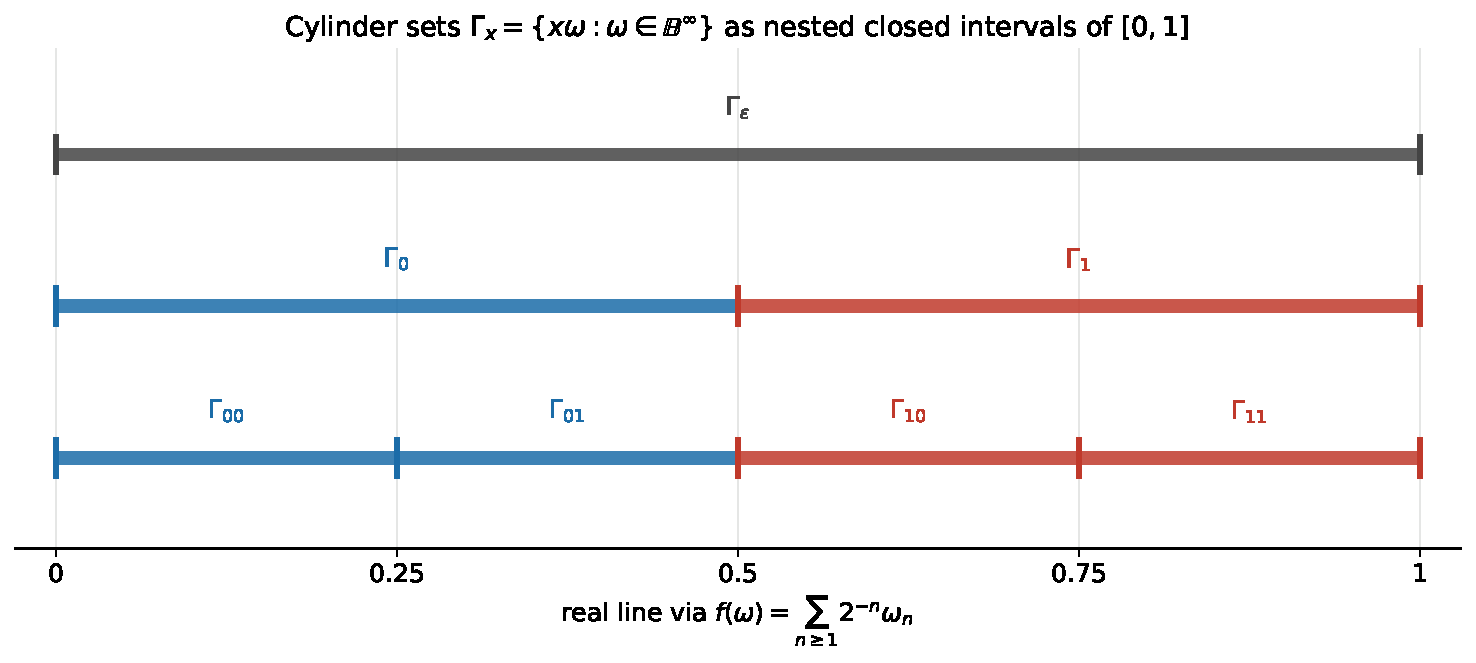
\includegraphics[width=0.82\textwidth]{fig_cylinder_sets}
\end{center}

\centering Fixing more bits of the prefix $x$ shrinks the interval
$f(\Gamma_x)$ by half each time.
\end{frame}

\begin{frame}{Reading the Cylinder-Set Picture}

\textbf{Plain English.} Every cylinder set $\Gamma_x$ corresponds to a
closed sub-interval of $[0,1]$ of width exactly $2^{-\len(x)}$: fixing
\emph{more} bits of the prefix $x$ shrinks the interval by half each time.
$\Gamma_\epsilon$ (the empty prefix, i.e.\ no constraint at all) is the
whole interval $[0,1]$. $\Gamma_0$ is the left half $[0,0.5]$ and $\Gamma_1$
is the right half $[0.5,1]$; $\Gamma_{00},\Gamma_{01}$ split $\Gamma_0$
into quarters, and likewise $\Gamma_{10},\Gamma_{11}$ split $\Gamma_1$.

\medskip
This nested-interval picture is exactly what will let us put a
\emph{probability measure} on $\Binf$ in Section 2.2, by assigning
probabilities to cylinder sets the same way we would assign lengths to
these intervals.
\end{frame}

%% ══════════════════════════════════════════════════════════════════════════
\begin{frame}[fragile]{Python: The Map $f$ and Example 2.1.9}

We verify Example 2.1.9 numerically. Each infinite sequence is approximated
by an explicit, long bit string (60 bits is far more than enough for
floating-point precision).

\begin{lstlisting}
def f(omega_bits):
    """f(omega) = sum_n 2^-n * omega_n, from an explicit (long,
    truncated) approximation `omega_bits` of the infinite sequence."""
    return sum(2 ** -(n + 1) * int(b) for n, b in enumerate(omega_bits))

zeros, ones = "0" * 60, "1" * 60
print("f(0^inf)    =", f(zeros))          # -> 0.0
print("f(010^inf)  =", f("01" + zeros))   # -> 0.25
print("f(110^inf)  =", f("11" + zeros))   # -> 0.75
print("f(10^inf)   =", f("1" + zeros))    # -> 0.5
print("f(01^inf)   =", f("0" + ones))     # -> 0.5  (same limit as above!)
print("f((01)^inf) =", f("01" * 30))      # -> 1/3
\end{lstlisting}

\textbf{Output matches Example 2.1.9 exactly}, including the subtle point
that $10^\infty$ and $01^\infty$ both map to $0.5$.
\end{frame}

\begin{frame}[fragile]{Python: Cylinder Sets as Intervals}

We confirm that the cylinder set $\Gamma_x$ corresponds to an interval of
width exactly $2^{-\len(x)}$.

\begin{lstlisting}
def cylinder_interval(x):
    """Gamma_x corresponds to [b(x)/2^len(x), (b(x)+1)/2^len(x)]."""
    if x == "":
        return (0.0, 1.0)
    n = len(x)
    lo = int(x, 2) / 2 ** n
    return (lo, lo + 2 ** (-n))

for x in ["", "0", "1", "01", "10", "011"]:
    lo, hi = cylinder_interval(x)
    print(f"Gamma_{x or 'eps'} = [{lo:.4f}, {hi:.4f}]  width={hi-lo:.4f}")
\end{lstlisting}

\textbf{Output:} widths are $1, 0.5, 0.5, 0.25, 0.25, 0.125$ respectively
--- exactly $2^{-\len(x)}$, confirming Remark 2.1.11.
\end{frame}

%% ══════════════════════════════════════════════════════════════════════════
\section{Summary}
%% ══════════════════════════════════════════════════════════════════════════

\begin{frame}{Section 2.1 Summary}
\begin{itemize}
  \item $\Bs=\bigcup_{n\geq0}\Bb^n$ is the set of all finite binary
    strings; $\Binf$ is the set of infinite binary sequences.
  \item The bijection $\bij{\cdot}:\Bs\to\mathbb{N}_0$,
    $\bij{x}=2^{\len(x)}+b(x)-1$, lets us treat strings and natural numbers
    interchangeably; $\bij{x}$ grows exponentially in $\len(x)$
    (Proposition 2.1.3).
  \item \textbf{Prefix-free} codeword sets make messages uniquely
    decodable without a delimiter (Theorem 2.1.7). The self-delimiting
    family $E_i$ trades code length for simplicity: $E_0$ costs
    $O(2^{\len(x)})$ bits, while $\overline{x}=E_1(x)$ and $x'=E_2(x)$ cost
    only $\len(x)+O(\log\len(x))$ bits.
  \item \textbf{Cylinder sets} $\Gamma_x=\{x\omega:\omega\in\Binf\}$ give
    $\Binf$ a geometric picture as nested closed intervals of $[0,1]$ of
    width $2^{-\len(x)}$, via the map
    $f(\omega)=\sum_{n\geq1}2^{-n}\omega_n$. This interval structure is the
    foundation on which Section 2.2 builds probability measures over
    infinite sequences.
\end{itemize}
\end{frame}

\end{document}
